\documentclass{article}
\usepackage[utf8]{inputenc}
\usepackage[spanish]{babel}
\usepackage{listings}
\usepackage{graphicx}
\graphicspath{ {images/} }
\usepackage{cite}
\usepackage{pstricks,pst-node}
\usepackage{schemata}

\begin{document}

\begin{titlepage}
    \begin{center}
        \vspace*{1cm}
            
        \Huge
        \textbf{Informe Final Parcial II}
            
        \vspace{0.5cm}
        \LARGE
        Entrega Final
            
        \vspace{1.5cm}
            
        \textbf{JUAN DIEGO ARIAS TORO}
            
        \vfill
            
        \vspace{0.8cm}
            
        \Large
        Despartamento de Ingeniería Electrónica y Telecomunicaciones\\
        Universidad de Antioquia\\
        Medellín\\
        Septiembre de 2021
            
    \end{center}
\end{titlepage}

\tableofcontents
\newpage
\section{Clases Implementadas}\label{intro}
La única clase implementada es la de la imagen, para a la cual maneja las rutas para encontrar las imágenes, y también la ruta para la escritura del archivo .txt, cuando ya tenga la imagen esta misma se encarga de recibir los valores de su alto y su ancho.

Esta misma contiene su constructor que será el cual nos entregará el los valores que se almacenarán en los atributos anteriormente mencionados.


\section{Esquema de tareas} \label{contenido}
\begin{center}
\begin{minipage}[c]{1\textwidth}
\schema{\schemabox{Clases}}{
        	\schemabox{
        		\schema{\schemabox{$\bullet$ Imagen}}
        	{
        	\schemabox{
    							\schema{\schemabox{$\bullet$ Ruta de la imagen}}{\schemabox{--Atributo Privado}\schemabox{--Tipo String}}}
    						\schemabox{
    							\schema{\schemabox{$\bullet$ Ruta del archivo .txt}}{\schemabox{--Atributo Privado}\schemabox{--Tipo String}}}
	        				\schemabox{
    							\schema{\schemabox{$\bullet$ Alto de la imagen}}{\schemabox{--Atributo Privado}\schemabox{--Tipo entero}}}
    						\schemabox{
    							\schema{\schemabox{$\bullet$ Ancho de la imagen}}{\schemabox{--Atributo Privado}\schemabox{--Tipo entero}}}
    						\schemabox{
    							\schema{\schemabox{$\bullet$Metodo Imagen}}{\schemabox{--Se debe seleccionar el archivo de lectura y el de escritura}\schemabox{--Toma los datos del ancho y del alto}\schemabox{--Constructor}}}
    						\schemabox{
    							\schema{\schemabox{$\bullet$Metodo de muestreo}}{\schemabox{--Toma secciones }\schemabox{--Modifica el tamaño de las secciones}\schemabox{--Duplica los tamaños de las muestras}}}
        		}
    		}
}
\end{minipage}
\end{center}
\section{Codigo y clases} \label{contenido}
\subsection{C++}
\begin{lstlisting}
#include <iostream>
#include <QImage>
#include <cmath>
#include <fstream>
using namespace std;
class imagen{
private:
    string ruta;
    int alto;
    int ancho;
    string rutaTXT;
public:
    imagen(string,string);
    void Muestreo();
};
imagen::imagen(string _rutaImagen,string _rutaTXT){
    ruta=_rutaImagen;
    rutaTXT=_rutaTXT;
    QImage ima(ruta.c_str());
    alto=ima.height();
    ancho=ima.width();
};
void imagen::Muestreo(){
    ofstream file;
    file.open(rutaTXT);
    QImage ima(ruta.c_str());
    int contador=0;
    double muestraX=ancho*0.125;
    double muestraY=alto*0.125;
    if(muestraX>=1||muestraY>=1){
        for(int i=(muestraY/2);i<alto;i+=(muestraY)){//alto
            for(int j=muestraX/2;j<ancho;j+=muestraX){//ancho
                file << to_string(ima.pixelColor(j,i).red())<<",";
                file << to_string(ima.pixelColor(j,i).green())<<",";
                file << to_string(ima.pixelColor(j,i).blue())<<",";
                contador++;
            }

        }
    }else{
        //sobremuestreo
        double avanceX=0;
        double avanceY=0;
        for(int i=0;i<8;i++){ //alto
            for(int j=0;j<8;j++){//ancho
                file << to_string(ima.pixelColor(floor(avanceX),floor(avanceY)).red())<<",";
                file << to_string(ima.pixelColor(floor(avanceX),floor(avanceY)).green())<<",";
                file << to_string(ima.pixelColor(floor(avanceX),floor(avanceY)).blue())<<",";
                contador++;
                avanceX=muestraX+avanceX;
            }
            avanceX=0;
            avanceY=muestraY+avanceY;
        }
    }
    cout<<ancho<<" x "<<alto<<"  muestreo culminado con EXITO"<<contador<<endl;
    file.close();
};
int main()
{
    string ruta="../pruebas1/flags/jap.jpg";
    string rutaTXT="../pruebas1/archivo.txt";
    QImage im(ruta.c_str());
    imagen bandera(ruta,rutaTXT);
    bandera.Muestreo();
    return 0;
}
\end{lstlisting}
\section{Circuito} \label{contenido}
\begin{figure}[h]
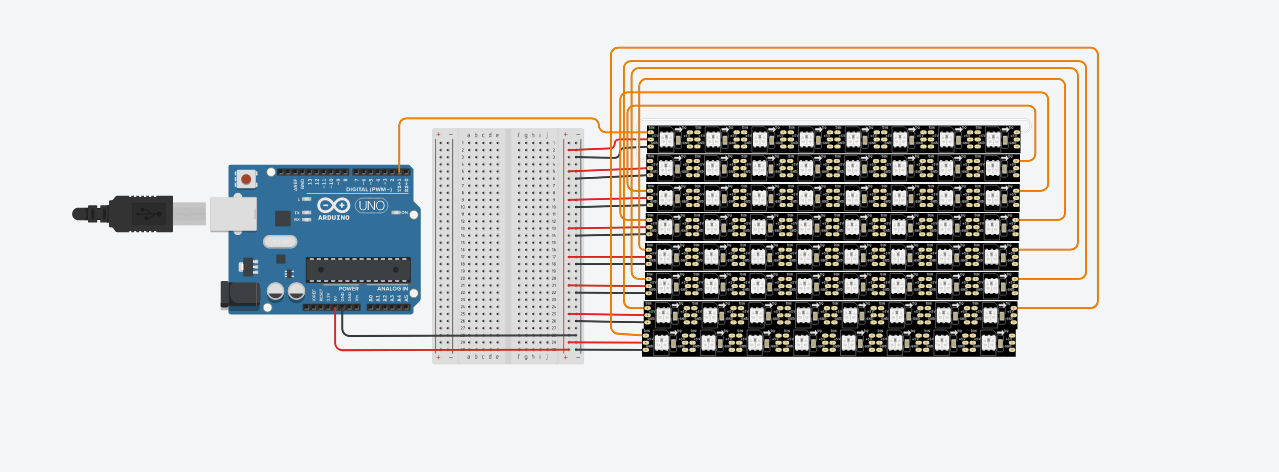
\includegraphics[width=15cm]{Circuito.png}
\end{figure}
La estructura se compone de una protoboard, un arduino y ocho tiras Neopixel de ocho LED cada una. Las tiras llevan una conexión al positivo y al negativo de la protoboard (el negativo y el positivo, lo define el usuario) a su vez, la protoboard lleva una conexión a la salida de 5 voltios del arduino y el negativo al GND del mismo.

A su vez la información es enviada por medio del puerto D1 del arduino directamente a las tiras LED, las cuales deben estar unidas por la salida de una, con la entrada de otra todo esto mediante cables.

\section{Problemas Presentados} \label{contenido}
\begin{itemize}
\item La ausencia de las librerias
\item El manejo de los objetos propios de la libreria QImages, no permita el manejo de operaciones directamente
\item No poder conectar directamente QT con el simulador de Tinkercad
\end{itemize}
\section{Manual de usuario} \label{contenido}
\begin{enumerate}
\item Descargar la imagen que desea tratar, guardandola en la carpeta Flags (es importante que la imagen sea tipo .jpg, de lo contrario no será leída por el programa).
\item Abrir el programa en QT y en este mismo ubicar la línea 61, ../pruebas1/flags/\textit{\textbf{NombreDeLaImagen}}.jpg en el espacio en negrita escribir el nombre de su imagen 
\item Ejecutar el programa con en botón que se encuentra en la izquierda inferior (un triángulo verde)
\item El programa le notificará si ha logrado transformar su imagen
\item Dirigirse en su explorador de archivos a la carpeta CodigoQt, pruebas1, archivo.txt. Allí encontrará una larga fila de números copialos todos hasta el último
\item Diríjase al simulador de Tinkercad al proyecto Parcial II informática, en;la seccion de codigo, en la línea 9, despues del igual y entre las llaves copie los números que le entrego el archivo .txt 
\end{enumerate}
\end{document}